\section{Self-energy}

\begin{framenologo}
  \frametitle{Self-energy}
  \tableofcontents[currentsection]
\end{framenologo}

\subsection{The concept}

\begin{frame}
  \frametitle{Self-energy}
  \framesubtitle{The concept}

  \begin{block}{Self-energies -- perturb the Hamiltonian}
    
    \begin{itemize}[<+->]
      \item A self-energy \emph{renormalises} the Hamiltonian
      \begin{equation*}
        \HH' = \HH + \SE
      \end{equation*}
      \item May describe wide variety of physical properties
      \begin{itemize}[<.->]
        \item Semi-infinity
        \item Local defects
        \item Absorbing potentials
        \item \dots
      \end{itemize}
      \item TranSiesta, self-energies are \emph{only} semi-infinite leads

      \item ! TBtrans allows custom (additional) self-energies, \emph{even} when calculating
      transport from DFT Hamiltonians
    \end{itemize}

  \end{block}

\end{frame}

\subsection{Semi-infinity}

\begin{frame}
  \frametitle{Self-energy}
  \framesubtitle{Semi-infinity}

  \begin{itemize}
    \item%
    Describes interaction of a system to a semi-infinite region
    
    \item%
    Self-energy calculations \emph{require} no more than nearest neighbour interactions between unit-cells

    \begin{align*}
      \SE_{\mrc 11}(E) &= \VV^\dagger\big[E+\im\eta-\HH\big]^{-1}\VV
      \\
      &\vdots
      \\
      \SE_{\mrc i1}(E) &= \VV^\dagger\big[E+\im\eta-\HH-\SE_{\mrc{i-1}1}(E)\big]^{-1}\VV
    \end{align*}

    Continue until $\SE_{\mrc i1}\approx\SE_{\mrc{i+1}1}$

    \begin{center}
      \animategraphics{.33}{../fig/inv-block_}{0}{17}
    \end{center}

  \end{itemize}
  
\end{frame}


\subsection{Bulk self-energy requirements}

\begin{frame}
  \frametitle{Self-energy}
  \framesubtitle{Semi-infinity -- which unit-cells?}

  \begin{center}
    \def\mysize{6pt}
    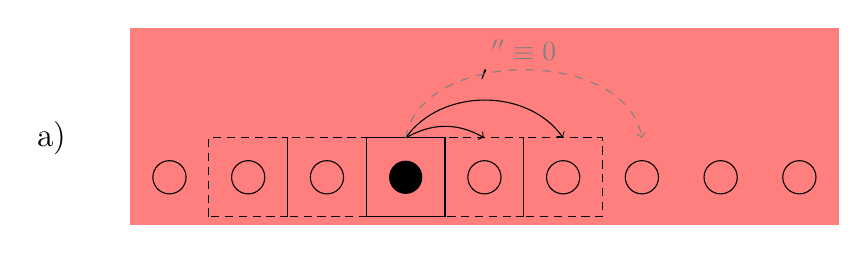
\begin{tikzpicture}
      \only<2->{
          \fill[red,opacity=.5] (-3,-.6) rectangle ++(9, 2.5);
      }
      \node[font=\large] at (-4,.5) {a)};
      \path (-3,-.5) rectangle ++(3,1);
      \path (3,-.5) rectangle ++(3,1);
      \draw[densely dashed] (-2,-.5) rectangle ++(1,1);
      \draw[densely dashed] (-1,-.5) rectangle ++(1,1);
      \draw (0,-.5) rectangle ++(1,1);
      \draw[densely dashed] (1,-.5) rectangle ++(1,1);
      \draw[densely dashed] (2,-.5) rectangle ++(1,1);
      \fill (.5,0) circle (\mysize);
      \foreach \x in {-2.5,-1.5,-.5,1.5,2.5,3.5,4.5,5.5} {
          \draw (\x,0) circle (\mysize);
      }

      \draw[->] (0.5,.5) to[out=30,in=150] node[above] {$\VV$} ++(1,0);
      \draw[->] (0.5,.5) to[out=55,in=125] node[above] {$\VV'$} ++(2,0);
      \draw[->,dashed,gray] (0.5,.5) to[out=80,in=100] node[above,gray] {$\VV''\equiv0$} ++(3,0);

    \end{tikzpicture}

    \vspace{4pt}

    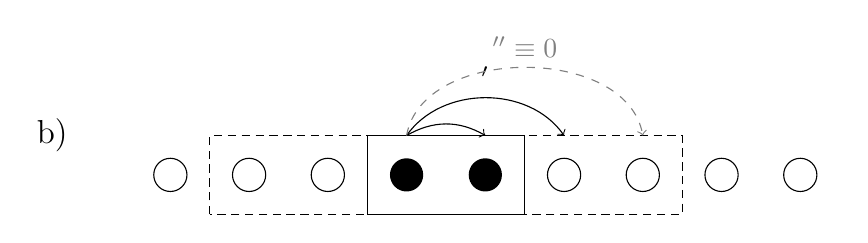
\begin{tikzpicture}
      \node[font=\large] at (-4,.5) {b)};
      \path (-3,-.5) rectangle ++(3,1);
      \path (3,-.5) rectangle ++(3,1);
      \draw[densely dashed] (-2,-.5) rectangle ++(2,1);
      \draw (0,-.5) rectangle ++(2,1);
      \draw[densely dashed] (2,-.5) rectangle ++(2,1);
      \fill (.5,0) circle (\mysize);
      \fill (1.5,0) circle (\mysize);
      \foreach \x in {-2.5,-1.5,-.5,2.5,3.5,4.5,5.5} {
          \draw (\x,0) circle (\mysize);
      }
      \draw[->] (0.5,.5) to[out=30,in=150] node[above] {$\VV$} ++(1,0);
      \draw[->] (0.5,.5) to[out=55,in=125] node[above] {$\VV'$} ++(2,0);
      \draw[->,dashed,gray] (0.5,.5) to[out=80,in=100] node[above,gray] {$\VV''\equiv0$} ++(3,0);
    \end{tikzpicture}

    \vspace{4pt}

    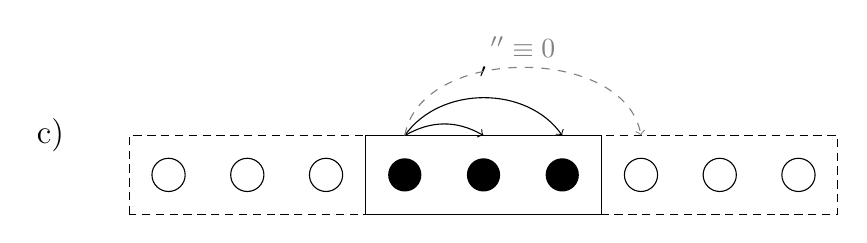
\begin{tikzpicture}
      \node[font=\large] at (-4,.5) {c)};
      \draw[densely dashed] (-3,-.5) rectangle ++(3,1);
      \draw (0,-.5) rectangle ++(3,1);
      \draw[densely dashed] (3,-.5) rectangle ++(3,1);
      \fill (.5,0) circle (\mysize);
      \fill (1.5,0) circle (\mysize);
      \fill (2.5,0) circle (\mysize);
      \foreach \x in {-2.5,-1.5,-.5,3.5,4.5,5.5} {
          \draw (\x,0) circle (\mysize);
      }
      \draw[->] (0.5,.5) to[out=30,in=150] node[above] {$\VV$} ++(1,0);
      \draw[->] (0.5,.5) to[out=55,in=125] node[above] {$\VV'$} ++(2,0);
      \draw[->,dashed,gray] (0.5,.5) to[out=80,in=100] node[above,gray] {$\VV''\equiv0$} ++(3,0);
    \end{tikzpicture}


    \vspace{5pt}

    This is \emph{only} a requirement along the semi-infinite direction!
  \end{center}

\end{frame}


\begin{frame}
  \frametitle{Self-energy}
  \framesubtitle{Semi-infinity -- rules}

  \tikzset{block/.style={
          shape=rectangle,draw,minimum size=.8cm},
      dd/.style={densely dotted},
      block dd/.style={block,dd},
  }
  \def\bsize{.8cm}

  \begin{block}{Rules for using self-energies}

    Coupling a \emph{bulk} electrode to a device requires(!) coupling region to behave
    \emph{bulk} as well. 

    \vspace{4pt}

    \begin{center}
      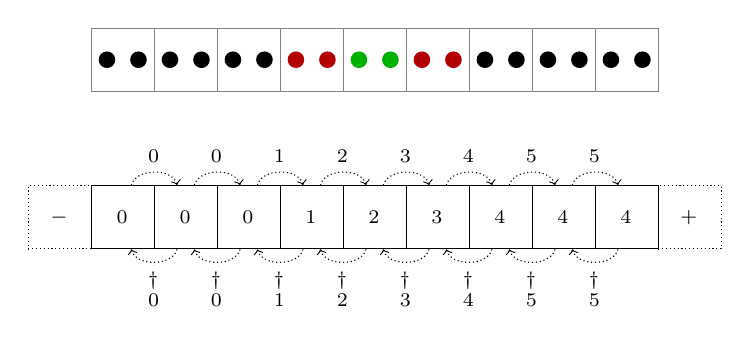
\begin{tikzpicture}

        \uncover<+->{
            \foreach \x in {0,1,2,3,4,5,6,7,8} {
                \def\tmpcol{black}
                \ifnum\x>2
                \def\tmpcol{red!70!black}
                \fi
                \ifnum\x>3
                \def\tmpcol{green!70!black}
                \fi
                \ifnum\x>4
                \def\tmpcol{red!70!black}
                \fi
                \ifnum\x>5
                \def\tmpcol{black}
                \fi
                \node[block,gray] at ({(\x-0.5)*\bsize},3*\bsize) {};

                \expandafter\fill\expandafter[\tmpcol] ({(\x-0.75)*\bsize},3*\bsize)
                circle (3pt);
                \expandafter\fill\expandafter[\tmpcol] ({(\x-0.25)*\bsize},3*\bsize)
                circle (3pt);

            }
        }
    
        \uncover<+->{
            \node[block dd] at (-1.5*\bsize,0.5*\bsize) {$\SE_{-}$};
            \foreach \x in {0,1,2,3,4,5,6,7,8} {
                \ifnum\x<3
                \def\tmpnum{0}
                \fi
                \ifnum\x>2
                \pgfmathparse{int(\x-2)}
                \edef\tmpnum{\pgfmathresult}
                \fi
                \ifnum\x>5
                \pgfmathparse{int(4)}
                \edef\tmpnum{\pgfmathresult}
                \fi
                \node[block] (A\x) at ({(\x-0.5)*\bsize},0.5*\bsize) {$\HH_\tmpnum$};
                \ifnum\x>0
                \pgfmathparse{int(\x-1)}
                \edef\xp{\pgfmathresult}
                \ifnum\x>6
                \pgfmathparse{int(5)}
                \edef\tmpnum{\pgfmathresult}
                \fi
                \draw[->,dd] (A\xp) to[out=75,in=105] node[above] {$\VV_\tmpnum$} (A\x);
                \draw[<-,dd] (A\xp) to[out=-75,in=-105] node[below] {$\VV^\dagger_\tmpnum$} (A\x);
                \fi
            }
            \node[block dd] at (8.5*\bsize,0.5*\bsize) {$\SE_{+}$};
        }
      \end{tikzpicture}

    \end{center}

    \vspace{-12pt}

    \begin{itemize}
      \item<+-> Remember that $\SE_{-/+}$ is a correction to the Hamiltonian (i.e.
      $\HH' = \HH + \SE$)
    \end{itemize}
  \end{block}

  \footnotesize
  \begin{columns}<+->
    \column{.25\textwidth}
    \begin{itemize}
      \item $\SE_-$ into 1st $\HH_0$?

      \begin{tikzpicture}
        \only<.>{
            \node[block,gray,fill=check] at (-0.5*\bsize,3*\bsize) {};
        }
        \uncover<.(1)->{
            \node[block,gray,fill=good] at (-0.5*\bsize,3*\bsize) {};
        }
        \foreach \x in {0.5,1.5,2.5} {
            \node[block,gray] at (\x*\bsize,3*\bsize) {};
        }
        \foreach \x in {0,1,2} {
            \fill[black] ({(\x-0.75)*\bsize},3*\bsize)
            circle (3pt)
            ({(\x-0.25)*\bsize},3*\bsize) circle (3pt);
        }
        \fill[red!70!black] (2.75*\bsize,3*\bsize)
        circle (3pt)
        (2.25*\bsize,3*\bsize) circle (3pt);
      \end{tikzpicture}
    \end{itemize}
    
    \column{.25\textwidth}
    \begin{itemize}
      \item $\SE_-$ into 2nd $\HH_0$?

      \begin{tikzpicture}
        \only<.>{
            \node[block,gray,fill=check] at (0.5*\bsize,3*\bsize) {};
        }
        \uncover<.(1)->{
            \node[block,gray,fill=good] at (0.5*\bsize,3*\bsize) {};
        }
        \foreach \x in {-0.5,1.5,2.5} {
            \node[block,gray] at (\x*\bsize,3*\bsize) {};
        }
        \foreach \x in {0,1,2} {
            \fill[black] ({(\x-0.75)*\bsize},3*\bsize)
            circle (3pt)
            ({(\x-0.25)*\bsize},3*\bsize)
            circle (3pt);
        }
        \fill[red!70!black] (2.75*\bsize,3*\bsize)
        circle (3pt)
        (2.25*\bsize,3*\bsize) circle (3pt);
      \end{tikzpicture}
    \end{itemize}

    \column{.25\textwidth}
    \begin{itemize}
      \item $\SE_-$ into 3rd $\HH_0$?

      \begin{tikzpicture}
        \only<.>{
            \node[block,gray,fill=check] at (1.5*\bsize,3*\bsize) {};
        }
        \uncover<.(1)->{
            \node[block,gray,fill=good] at (1.5*\bsize,3*\bsize) {};
        }
        \foreach \x in {-0.5,0.5,2.5} {
            \node[block,gray] at (\x*\bsize,3*\bsize) {};
        }
        \foreach \x in {0,1,2} {
            \fill[black] ({(\x-0.75)*\bsize},3*\bsize)
            circle (3pt)
            ({(\x-0.25)*\bsize},3*\bsize) circle (3pt);
        }
        \fill[red!70!black] (2.75*\bsize,3*\bsize)
        circle (3pt)
        (2.25*\bsize,3*\bsize) circle (3pt);
      \end{tikzpicture}
    \end{itemize}

    \column{0.25\textwidth}
    \begin{itemize}
      \item $\SE_-$ into $\HH_1$?

      \begin{tikzpicture}
        \only<.>{
            \node[block,gray,fill=check] at (2.5*\bsize,3*\bsize) {};
        }
        \uncover<.(1)->{
            \node[block,gray,fill=bad] at (2.5*\bsize,3*\bsize) {};
        }
        \foreach \x in {-0.5,0.5,1.5} {
            \node[block,gray] at (\x*\bsize,3*\bsize) {};
        }
        \foreach \x in {0,1,2} {
            \fill[black] ({(\x-0.75)*\bsize},3*\bsize)
            circle (3pt)
            ({(\x-0.25)*\bsize},3*\bsize) circle (3pt);
        }
        \fill[red!70!black] (2.75*\bsize,3*\bsize)
        circle (3pt)
        (2.25*\bsize,3*\bsize) circle (3pt);
      \end{tikzpicture}
    \end{itemize}

  \end{columns}

\end{frame}
